\documentclass[12pt,preprint]{aastex}
\usepackage{amssymb,amsmath}
%\usepackage{color,hyperref}
%\definecolor{linkcolor}{rgb}{0,0,0.25}
%\hypersetup{
%  colorlinks=true,        % false: boxed links; true: colored links
%  linkcolor=linkcolor,    % color of internal links
%  citecolor=linkcolor,    % color of links to bibliography
%  filecolor=linkcolor,    % color of file links
%  urlcolor=linkcolor      % color of external links
%}
\setlength{\emergencystretch}{2em}%No overflowing references
\newcommand{\ie}{i.e.}
\newcommand{\etal}{et al.}
\newcommand{\eg}{e.g.}
\newcommand{\eqnname}{equation}
\newcommand{\figurenames}{\figurename s}
\newcommand{\sectionname}{$\mathsection$}
\newcommand{\tvector}[1]{\boldsymbol{\vec{#1}}}
\newcommand{\vx}{\tvector{x}}
\newcommand{\vv}{\tvector{v}}

\begin{document}

\title{Title}
\author{Jo~Bovy}%\altaffilmark{1,2}}
\affil{Center for Cosmology and Particle Physics, Department of Physics, New York University, 4 Washington Place, New York, NY 10003, USA}
\email{jb2777@nyu.edu}
%\altaffiltext{1}{Center for Cosmology and Particle Physics, Department of Physics,
%  New York University, 4 Washington Place, New York, NY 10003, USA}
%\altaffiltext{2}{Correspondence should be addressed to jo.bovy@nyu.edu~.}

\begin{abstract}
Various dynamical scenarios related to the Milky Way's bar or spiral
structure have been proposed to explain the existence of moving
groups---clumps of co-moving stars---in the Solar neighborhood. Since
the observed pattern of moving groups is very sensitive to the
properties of the non-axisymmetric feature that creates them, these
moving groups can be a powerful tool in constraining the dynamical
structure of the inner Milky Way. However, at present the various
models are hard to confirm and distinguish with observations of the
local Galactic neighborhood. We show that future programs that survey
the Milky Way disk's kinematics on a more global scale can distinguish
between these models. By integrating orbits of stars in various
steady-state and transient bar and spiral structure potentials that
produce the pattern of moving groups observed in the Solar
neighborhood, we predict the velocity distribution as a function of
location in the Galactic disk. We identify the locations that
distinguish most clearly between the various scenarios. Future
infrared radial velocity surveys can probe the velocity distribution
at these locations. We predict the distribution of radial velocities
that can be directly compared to observations to establish the origin
of the moving groups and to constrain the structural and dynamical
parameters of the non-axisymmetric Milky Way potential.
\end{abstract}

\keywords{
  Galaxy: bulge
  ---  
  Galaxy: disk
  ---
  Galaxy: evolution
  ---
  Galaxy: fundamental parameters
  ---
  Galaxy: kinematics and dynamics
  ---
  Galaxy: structure
}

\section{Introduction}




\section{Methodology}

We follow Dehnen's approach \citep{dehnen00a}.


\subsection{Bar potential}


\begin{thebibliography}{}

\bibitem[{{Binney} \& {Tremaine}(2008)}]{binneytremaine}
{Binney},~J. \& {Tremaine},~S., 2008, {Galactic Dynamics: Second Edition}
  (Princeton University Press)

\bibitem[Bovy, Hogg, \& Roweis(2009)]{Bovy09a} Bovy,~J., Hogg,~D.~W., \& Roweis,~S.~T., 2009,
  \apj, 700, 1794

\bibitem[Dehnen(2000)]{dehnen00a}
  Dehnen,~W., 2000, \aj, 119, 800

\end{thebibliography}


\clearpage
\begin{figure}
\includegraphics[width=0.5\textwidth]{veldist.eps}
\caption{observed}\label{fig:obs}
\end{figure}

\clearpage
\begin{figure}
\includegraphics[width=\textwidth]{rphi2d.ps}
\caption{2D}\label{fig:rphi2d}
\end{figure}

\clearpage
\begin{figure}
\includegraphics[width=\textwidth]{rphi1d.ps}\\
\includegraphics[width=\textwidth]{rphi1d2.ps}
\caption{1D}\label{fig:rphi1d}
\end{figure}

\clearpage
\begin{figure}
\includegraphics[width=0.5\textwidth]{detecta.ps}
\includegraphics[width=0.5\textwidth]{detectb.ps}
\caption{detect}\label{fig:detect}
\end{figure}

\clearpage
\begin{figure}
\includegraphics[width=0.5\textwidth]{distuncertain.ps}
\includegraphics[width=0.5\textwidth]{df.ps}\\
\includegraphics[width=0.5\textwidth]{slope.ps}
\includegraphics[width=0.5\textwidth]{barstrength.ps}
\caption{1dvar}\label{fig:1dvar}
\end{figure}



\end{document}
